\section{Probability theory}

Data uncertainty, and more generally uncertainty, is linked with confidence.
Indeed, the confidence level that one can give to data depends on its uncertainty.
The more uncertain value is, the less trust it can be placed in it.
However, it is rather difficult to put exact numbers on this confidence level.
A strategy used by experts to formalise this confidence level, and thus the uncertainty, is to use probability distributions.

In this section, we thus introduce the necessary concepts of these distributions.
We first describe the concept of random variables in probability theory.
Then we describe what a probability distribution is and the properties that will be used in this thesis.
Finally, we will explain the distributions used in this thesis.

\subsection{Random variables}

\paragraph{Definition}
The three base elements of the probability theory are: an outcome, an event, and a sample space.
An outcome is the occurrence of a random phenomenon.
An event is a set of outcomes, and a sample space $S$ is the set of all possible outcomes.
Let us take an example: the rolling of two dice.
$i$ denotes the result of one die and $j$ the result of the other.
An example of an outcome is the result of a roll, like the pair (2, 6).
An event could contain all outcomes where both dice have an even result: $E = \{ (i,j) \mid i,j \in \{2, 4, 6\}\}$.
The sample space of our example is this equals to: $S_1 = \{ (i,j) \mid i,j \in \{1, 2, \dots , 6\} \}$.
We thus have: 

A random variable is a function from the sample space $S$ to $\mathds{R}$.
In our example, we can define two random variables $X$ and $Y$ that represent, respectively, the minimum of the two dice and the sum of the two.
We have thus: $X= min(i, j)$ and $Y= i + j$.

\paragraph{Discrete and continuous}
Random variable can be either discrete or continuous.
For discrete random variables, we can list all the events of the sample space, whereas we cannot for continuous ones.
For example, it is possible to list all results of the rolling of $n$ dice, $n \in \mathds{N}$.
But we cannot list all possible temperatures of a room (if we consider that we have an infinite precision).

\paragraph{Independence and disjoint}
Independence and joint are defined at the event level.
Two events are independent if the probability of occurrence of one does not impact the probability of occurrence of the others.
Two events are disjoint if and only if they do not share any outcome.
Mathematically speaking, events $A$ and $B$ are independent if and only if $P(A \cap B) = P(A) * P(B)$, and they are disjoint if and only if $P(A \cap B) = P(A) * P(B)$.

\subsection{Distribution}
A probability distribution of a random variable $X$ is a function that gives the probability that $X$ takes on the values $x$, for all possible values of the sample space.
Here, we can distinguish two cases: discrete and continuous distributions.
A distribution is said discrete when it is based on a discrete random variable, and continuous when the random variable is continuous.

The difference that will interest us in this thesis between the two is how they compute the probability, and thus the confidence level.
For discrete distributions, the probability that $X=x$ corresponds to the result of the function.
By definition, the probability that the random variable is inferior to a vale $x$ is thus equals to the sum of probability for $X < x$.

Contrary, for continuous distribution, the probability is mapped to the area under the function that which defines the probability distribution, \ie the integral of the function.
For example, the confidence that a given uncertain value is greater than zero is the surface under the function $f(x)$ for any $f(x) \mid f(x) > 0$. 
As the area under a precise point is null, the probability that a continuous random variable equals $x$ is zero.


\subsection{Distribution used in this thesis}

\begin{figure*}
    \centering
    \subfloat[Gaussian] {
        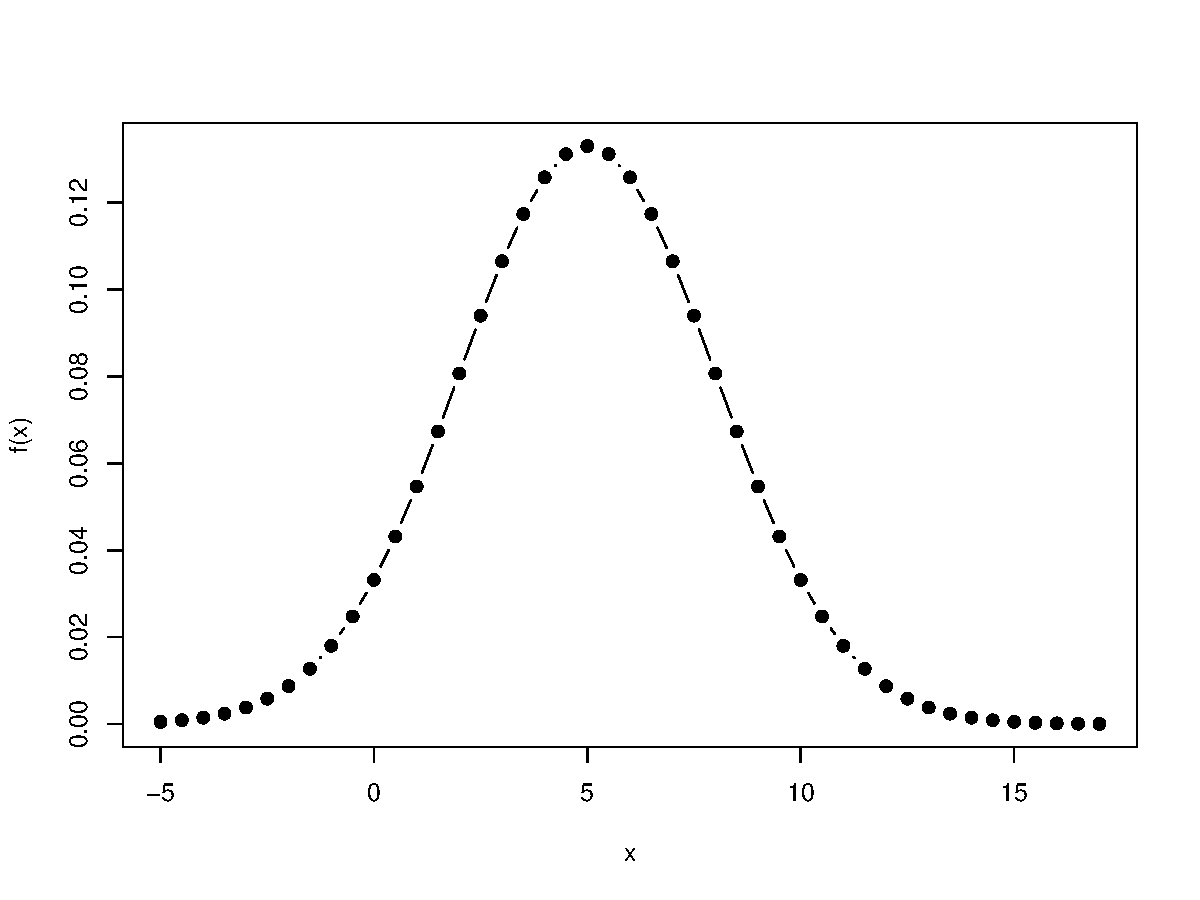
\includegraphics[width=.22\linewidth]{img/chapt-background/proba/Gaussian}
        \label{fig:back:proba:gauss}
    }
    \hfill
  	\subfloat[Rayleigh] {
        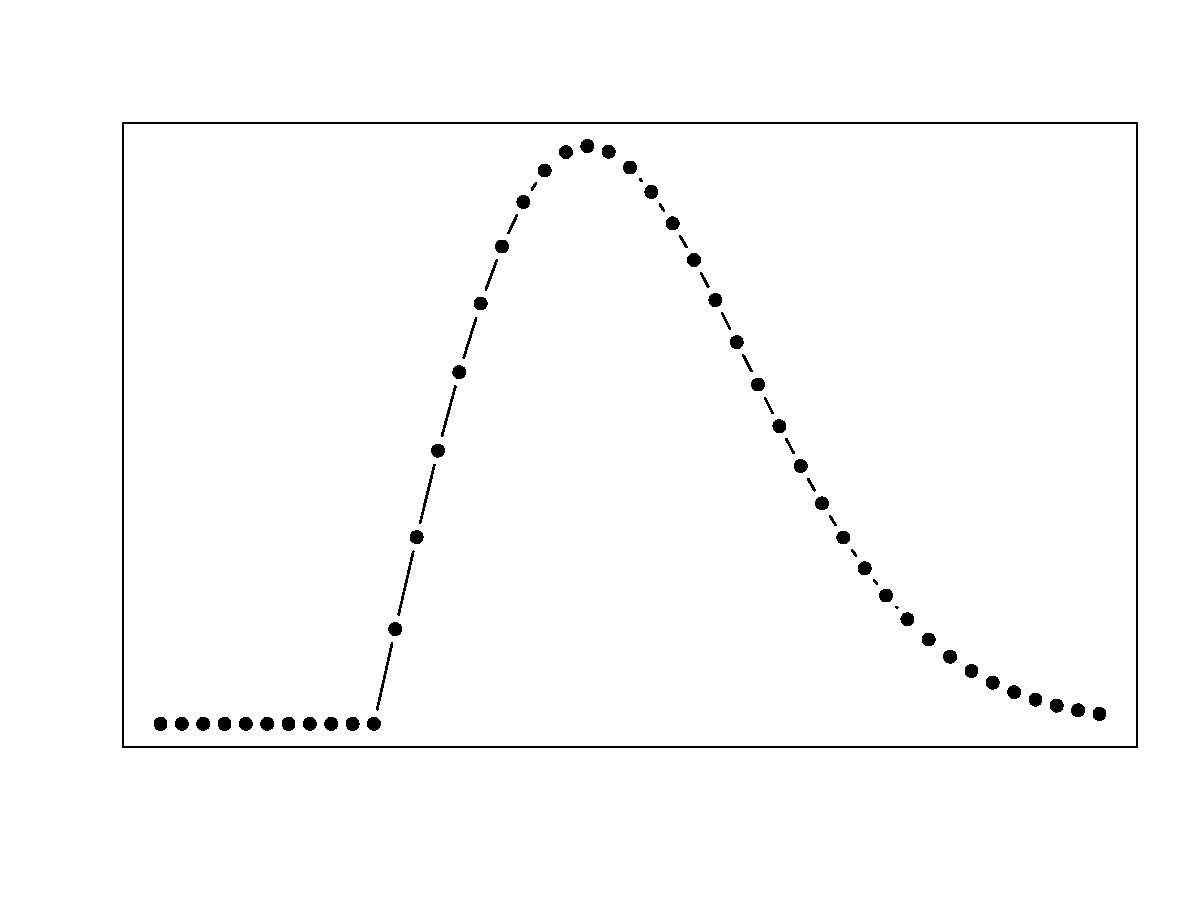
\includegraphics[width=.22\linewidth]{img/chapt-background/proba/Rayleigh}
        \label{fig:back:proba:ray}
    }
    \hfill
  	\subfloat[binomial] {
        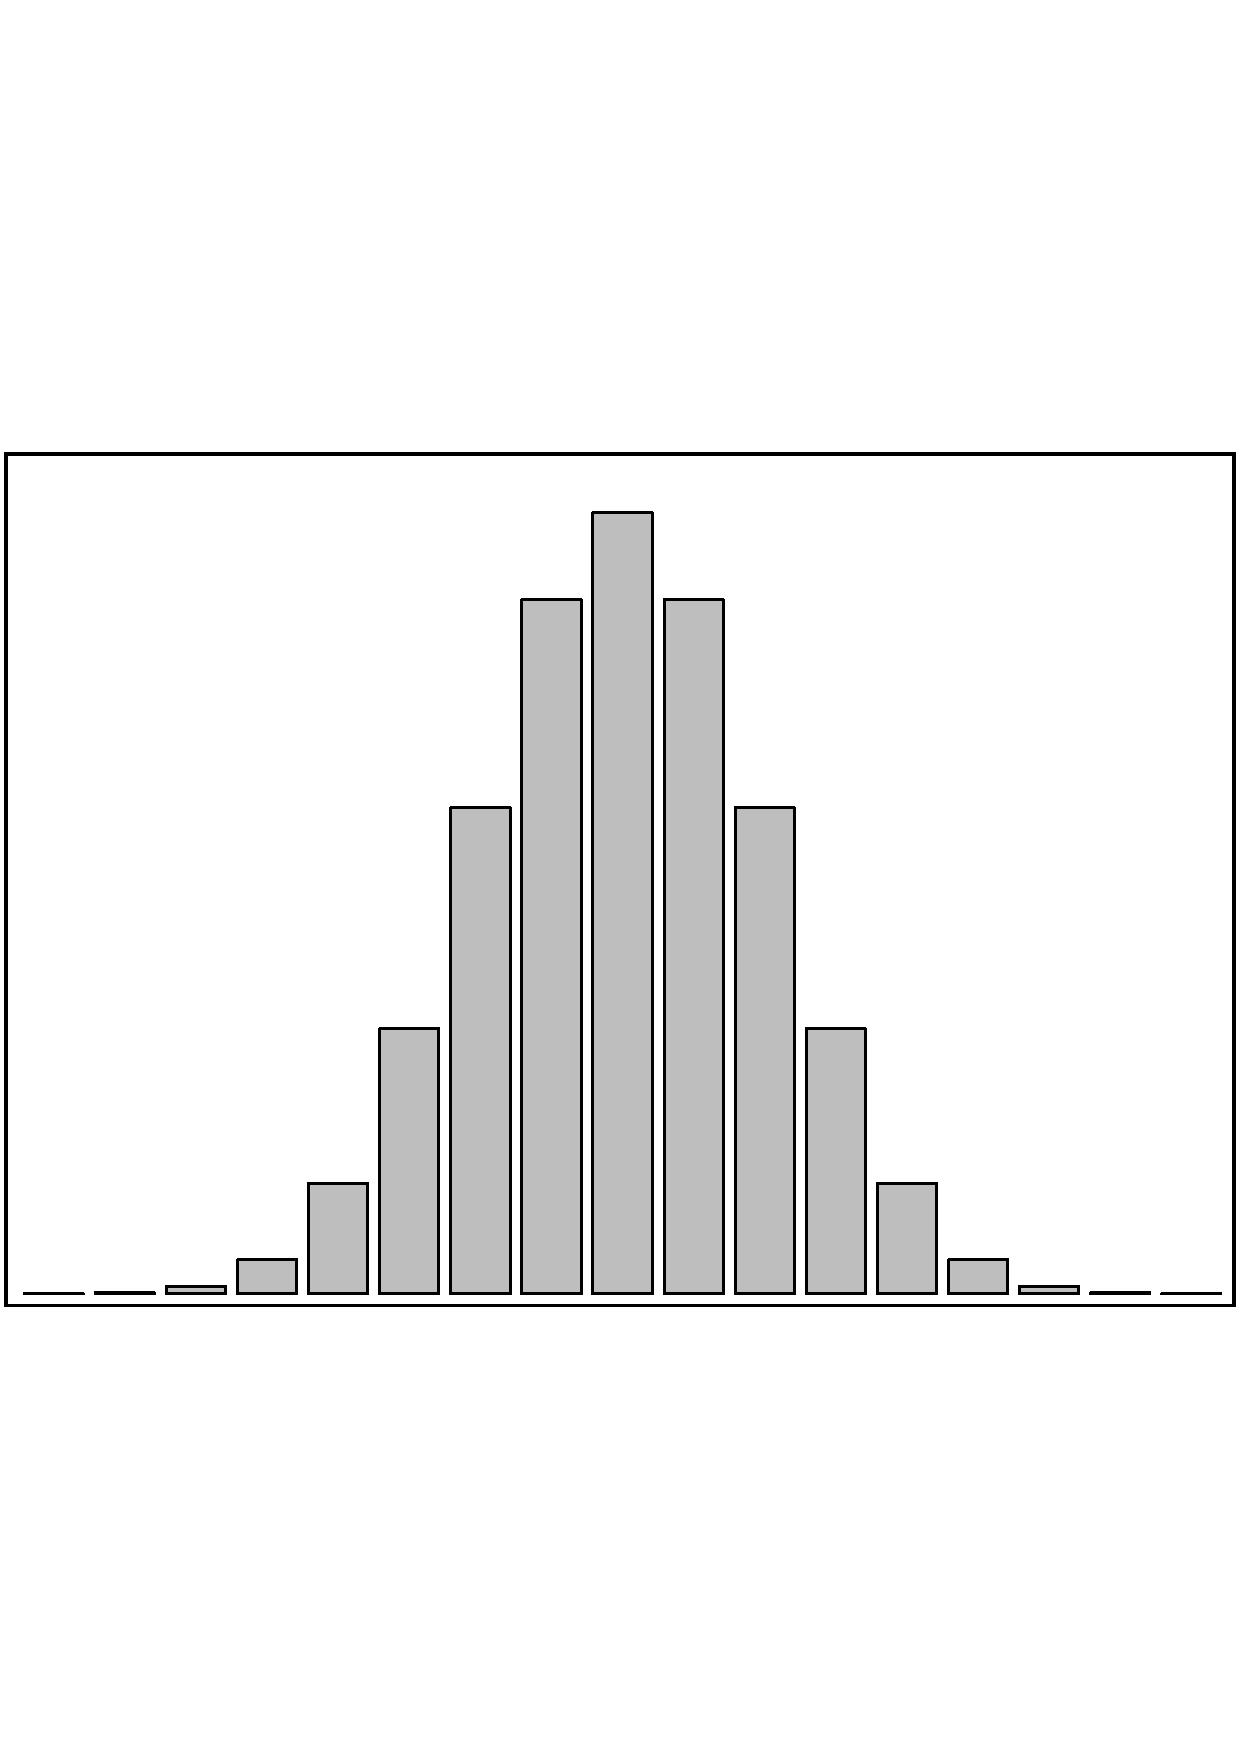
\includegraphics[width=.22\linewidth]{img/chapt-background/proba/binomial}
        \label{fig:back:proba:binom}
    }
    \hfill
    \subfloat[Dirac delta function] {
        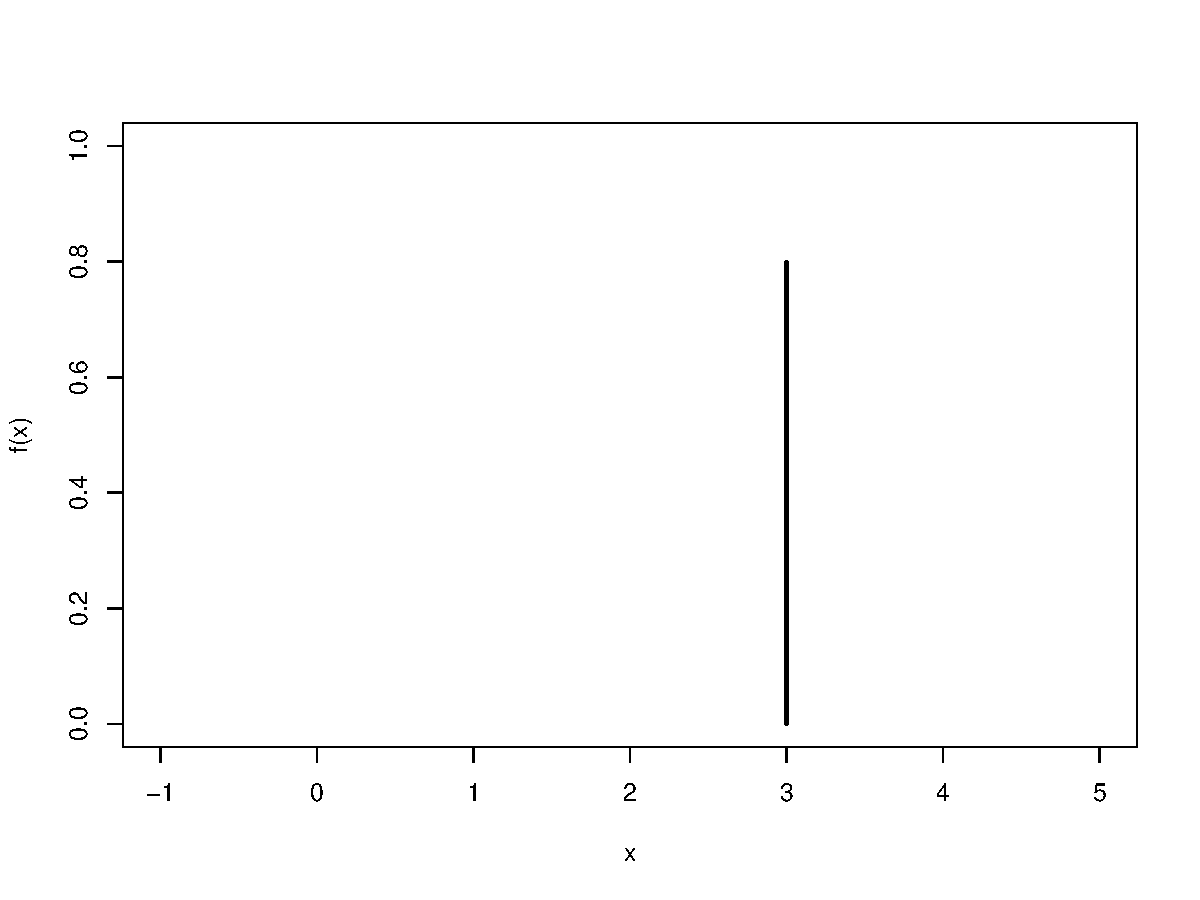
\includegraphics[width=.22\linewidth]{img/chapt-background/proba/dirac}
        \label{fig:back:proba:dirac}
    }
    \caption{Probability distributions used in this thesis}
    \label{fig:back:proba:examples}
\end{figure*}

Probability distributions have proven their ability to represent uncertain data.
Among the existing distributions, in this thesis, we use on five of them: Gaussian (or Normal) distribution, Rayleigh distribution, binomial distribution, Bernoulli distribution and the Dirac delta function.
The Gaussian and the Rayleigh distributions will represent continuous distributions.
The Bernoulli and the binomial one represent discrete distributions.
Finally, the Dirac delta function can represent the confidence level of exactly one value.

\paragraph{Bernoulli distribution}
Bernoulli distribution represents the distribution of a binary phenomenon.
One well-known example is the flip of a fair coin.
Bernoulli($p$) denotes a random variable that equals 1 with a probability of $p$ and 0 with a probability of $(1 - p)$.
Following the coin example, 1 can represent the head and 0 tail.

\paragraph{Binomial distribution}
The binomial distribution represents the probability of success of a binary phenomenon over a set of trials.
Figure~\ref{fig:back:proba:binom} illustrates an example of a Binomial distribution.
It is defined by two parameters: $n$ and $p$.
$n$ is the number of trials done and $p$ the probability of success.
By definition, it is defined over a discrete domain, more specifically on the set of natural number $\mathds{N}$.
In this case, the confidence level corresponds to the values of the function.

It has been proven that this distribution is similar to a Gaussian distribution in certain cases~\cite{box2005}.
If the domain definition can be changed from discrete to continuous, a binomial distribution can be approximated by a Gaussian distribution. 

\paragraph{Gaussian (or Normal) distribution}
The Gaussian distribution, commonly referred to as normal distribution, is the most general probability distribution.
For example, the International Bureau of Weights and Measures encourages the use of this distribution to quantify the uncertainty of measured values~\cite{metrology2008evaluation}.
It is defined by two parameters: a mean and a variance.
The distribution is defined on a continuous domain: $]-\infty; +\infty[$.
An example of this distribution is illustrated in Figure~\ref{fig:back:proba:gauss}.

\paragraph{Rayleigh distribution}
Another distribution defined on a continuous domain ($[0; +\infty[$) is the Rayleigh distribution.
It is often used for GPS positions~\cite{bornholt2013abstractions}.
This distribution is defined using a unique parameter: a variance.
We depict an example of this distribution in \Cref{fig:back:proba:ray}.

\paragraph{Dirac delta function}
The Dirac delta function is defined as a probability function with $f(x) = +\infty$ for $x=0$ and $f(x) = 0$ for all the other points.
To represent other values than zero, the following variable substitution can be used $x = x - a$,  where.
We call $a$ the shifting value.
By definition, the integral of this function on the whole domain definition is equal to 1.
As it is considered as a continuous distribution, confidence is mapped to the integral of the function.
By applying a coefficient, we can modify the value of this integral, \eg to have 0.8 as the integral.
We define this probability distribution using two parameters a coefficient and a shifting value.
An example of this probability distribution is shown in Figure~\ref{fig:back:proba:dirac}.
Conventionally, the Dirac function is represented as a vertical line that stops at the coefficient.
The figure shows a Dirac function with a coefficient of 0.8 and a shifting value of 3.
As it is defined on a single value, this distribution can be used for any numbers.
This distribution can be used to represent uncertainty that is due to human errors.